\documentclass[a4paper, 12pt]{article}


% Packages
\usepackage{multirow} 
\usepackage{booktabs} 
\usepackage{graphicx} 
\usepackage{graphics}
\usepackage{setspace}
\usepackage{float}
\usepackage{fancyhdr}
\usepackage[colorlinks,linkcolor=bleudefrance, citecolor=bleudefrance,urlcolor=magenta,
bookmarks=false,hypertexnames=true]{hyperref}
\usepackage{enumerate}
\usepackage{enumitem}
\usepackage{natbib}
\usepackage{amsmath,amssymb,amsthm}
\usepackage[left=1in,right=1in,top=0.8in,bottom=1in]{geometry}
\usepackage{titlesec}
\usepackage{lscape}
\usepackage[table,xcdraw]{xcolor}
\usepackage{chngcntr}

% Theorems
\newtheorem{mec}{Mechanism}
\newtheorem{hyp}{Hypothesis} 
\newcounter{subhyp} 
\newcommand{\subhyp}{ 
	\setcounter{subhyp}{0} 
	\renewcommand\thehyp{\protect\stepcounter{subhyp}% 
		\arabic{hyp}\alph{subhyp}\protect\addtocounter{hyp}{-1}} 
} 
\newcommand{\normhyp}{ 
	\renewcommand\thehyp{\arabic{hyp}} 
	\stepcounter{hyp} 
} 




\definecolor{bleudefrance}{rgb}{0.19, 0.55, 0.91}


\newcommand{\eqname}[1]{\tag*{#1}}% Tag equation with name

\author{Valentina Gonzalez-Rostani \\ email \href{mailto:mag384@pitt.edu}{mag384@pitt.edu} }

\begin{document}



\title{ \huge Tips for using \LaTeX}
\vspace{1in}
\date{\today}
\maketitle

\section{Welcome!}
Hi! This document is just a brief guide for beginners in $\LaTeX$. I hope you enjoy it. I am sharing the link to the overleaf so you can see both the pdf and the main.txt. Also, in the pdf, you can see code that I include using verbatim. 

This document proceeds as follows. I start by providing some insights about the steps you should follow to download $\LaTeX$ on your computer. This is not a necessary step because you can use overleaf, and it works very well. Then I briefly explain that every document has a preamble, and depending on what you plan to write, it requires some packages. Then, I present some of the tips that you need to know about the document's body. Sections 5 and 6 give basic insights about how to add figures and tables. Next, section 7 presents how to write equations, matrix, and basics math. This section is important because even if you use markdown, you will write math using this language. Then, section 8 explains how to cite and build your references. Finally, this guide ends by suggesting some links where you find more information and examples of documents that I wrote using $\LaTeX$. 

Tip 1: Have fun learning $\LaTeX$!
\section{Download the software}

There are many ways to use $\LaTeX$, one is by using overleaf, and the other is to use a software in your computer. The advantage of using overleaf is that you can collaborate and work at the same time in the file. 

If you want to install in your PC you will need two programs (example that I use - Im window user): 
\begin{itemize}
	\item \href{https://www.texstudio.org/}{Tex studio}
	\item \href{https://miktex.org/download}{Miktex}
\end{itemize}

We use the interface texstudio, but we need miktex installed to make everything work. 

Depending on your software there are different instructions to follow: 
\begin{itemize}
    \item \href{http://www.tug.org/mactex/}{Mac Instructions}
    \item \href{https://www.math.ucsd.edu/~wcheung/texforwindows.html}{Window Instructions}
\end{itemize}

\section{Beginning of the file}
\subsection*{Preamble}
All $\LaTeX$ files have a preamble where we define the format of the file, and we call the packages that we need.

The first line is always defining the document class. Following there is an example, this is an article and the size is 11pt.

\begin{verbatim}
\documentclass[a4paper, 11pt]{article}
\title{Cartesian closed categories and the price of eggs}
\author{Jane Doe}
\date{September 1994}
\begin{document}
\maketitle
Hello world!
\end{document}
\end{verbatim}

\subsection*{Packages}
Before the ``begin document'' we also should define format of the text that we will use, for example: 

\begin{verbatim}
\usepackage[colorlinks,linkcolor=bleudefrance, citecolor=bleudefrance,urlcolor=magenta,
bookmarks=false,hypertexnames=true]{hyperref}
\end{verbatim}

This command says, use the package colorlinks, and defines the color of the links, and references. We can change it to black if we prefer no color. 

\vspace{0.2in}
\textbf{Important tip} $\rightarrow$ It is useful to be very organized with the packages and maybe add a comment saying why you include it. This is a way to avoid having multiple packages without knowing why they are there. A confession: I am not super organized, but I am trying to apply this tip for myself. 
\vspace{0.2in}


Another example before ``begin document'' is to create some commands such as:
\begin{verbatim}
\newtheorem{mec}{Mechanism}
\newtheorem{hyp}{Hypothesis} 
\newcounter{subhyp} 
\newcommand{\subhyp}{ 
\setcounter{subhyp}{0} 
\renewcommand\thehyp{\protect\stepcounter{subhyp}% 
\arabic{hyp}\alph{subhyp}\protect\addtocounter{hyp}{-1}} 
} 
\newcommand{\normhyp}{ 
\renewcommand\thehyp{\arabic{hyp}} 
\stepcounter{hyp} 
} 
\end{verbatim}

These lines basically define a command. In other words, you are creating a command, so you can call the command later. Then in the body of the document these commands will look like this: 

\begin{hyp}
	Here you should write the hypothesis 1. The numbers are automatically assigned.
\label{hi}
\end{hyp}

\begin{hyp}
	Here you should write the hypothesis 2. The numbers are automatically assigned.
\label{hiworld}
\end{hyp}

Then in the text, when you want to call your hypothesis you will write something like this: As I mentioned in the hypothesis \ref{hi} ....


\section{Body of the document}
\subsection*{Sections}
Every document may have \textbf{sections}, subsections, and subsubsections. We initiate the sections by writing:

\begin{verbatim}
\section{Name of the section here}
\subsection{Name}
\end{verbatim}

If you do not want numbers in the sections, then you have to add $*$ before the name: 

\begin{verbatim}
\section*{Name of the section here}
\subsection*{Name}
\end{verbatim}

\subsection*{Itemize}

If we want to \textbf{enumerate} or define items we will use this command:

\begin{verbatim}
\begin{itemize}
\item X
\item Y
\end{itemize}



\begin{enumerate}
\item X
\item Y
\end{enumerate}

\end{verbatim}

\begin{itemize}
	\item X
	\item Y
\end{itemize}
If we want numbers we should write
\begin{enumerate}
	\item X
	\item Y
\end{enumerate}

\subsection*{Footnote}
When we want to define a \textbf{footnote} we should write the following command right after the place where the footnote should start:\footnote{This is a footnote} 

\begin{verbatim}
I will define a footnote right here\footnote{Hola}
\end{verbatim}

\subsection*{Format}
If we want to use: 
\begin{itemize}
	\item \textbf{Bold} $\rightarrow$ Ctrl + B or textbf
	\item \textit{Italic} $\rightarrow$ Ctrl + I or textit
	\item \underline{Underline} $\rightarrow$ underline
	\item Ctrl + U will make the selected words as capital letters. (it works in overleaf)
\end{itemize}
\begin{verbatim}
\textbf{Bold}
\textit{Italic}
\underline{Underline}
\end{verbatim}

Also if you need you can define color to the text: like \textcolor{red}{this}



\begin{verbatim}
\textcolor{red}{text with color here}
\textcolor{blue}{text with color here}
\textcolor{green}{text with color here}
\end{verbatim}

\subsection*{Spacing}
\begin{verbatim}
Double:	\doublespacing
1.5: \onehalfspacing
single: \begin{singlespace} and then \end{singlespace}
\end{verbatim}

\section{Figures}
To incorporate a figure in your \LaTeX you should have them in the same file or in the cloud. If you forget this step the file will not compile. 

Following I write some examples: 

\begin{verbatim}
\begin{figure}[h]
\caption{Wage distribution (kernel density estimation)}
\includegraphics[scale=0.50]{gyc.png}
\label{fig:gyc}
\centering
\end{figure}
\end{verbatim}

\begin{figure}[h]
\caption{This is an example of a title of a figure}
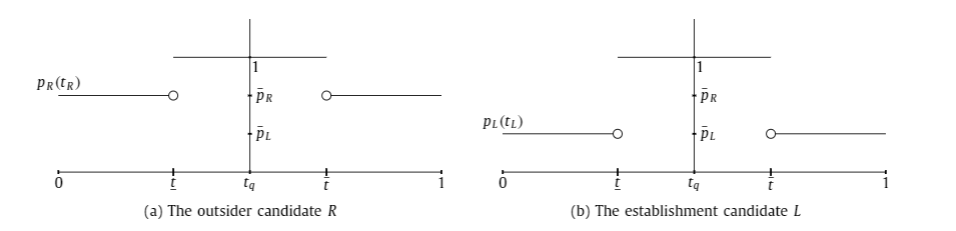
\includegraphics[scale=1]{comitment.png}
\label{example}
\centering
\end{figure}

\begin{itemize}
	\item caption $\rightarrow$ refers to the title of the figure
	\item label $\rightarrow$ this is hidden in the pdf, but this is useful to call the figure. Then if you want to talk about it you will write: \begin{verbatim}
	\ref{fig:gyc}
	\end{verbatim}
	\item centering $\rightarrow$ the figure will be centered
\end{itemize}
\section{Tables}
Tables seem very difficult but there are some tips to overcome this complexity. 

\begin{itemize}
	\item If you use stata and you are running a regression, you can export directly from stata and with one line you will have your regression table. Inside the parenthesis you should write the name of the file that you export from Stata
	
	\begin{verbatim}
	\input{Summary.tex}
	\end{verbatim}
	
	\item If you want to create a table a magic trick is to use a web page (see \href{https://www.tablesgenerator.com/latex_tables}{link}). There I copy and paste from excel the table that I want and this generate a perfect code. 
	
		\begin{verbatim}
% Please add the following required packages to your document preamble:
% \usepackage{graphicx}
\begin{table}[]
\centering
\caption{Example}
\label{undefined}
\resizebox{\textwidth}{!}{%
\begin{tabular}{|l|l|l|}
\hline
& \textbf{Column 1} & \textbf{Column 2} \\ \hline
\textbf{Raw 1} & X                 & Y                 \\ \hline
\textbf{Raw 2} & Z                 & W                 \\ \hline
\end{tabular}%
}
\end{table}
	\end{verbatim}
\end{itemize}

% Please add the following required packages to your document preamble:
% \usepackage{graphicx}
\begin{table}[H]
	\centering
	\caption{Example}
	\label{undefined}
		\begin{tabular}{|l|l|l|}
			\hline
			& \textbf{Column 1} & \textbf{Column 2} \\ \hline
			\textbf{Raw 1} & X                 & Y                 \\ \hline
			\textbf{Raw 2} & Z                 & W                 \\ \hline
		\end{tabular}
\end{table}

\section{Math}
As we all were expecting, the most important (and funniest) section arrived: how to write math!

$\LaTeX$ is great for writing Math but you need to be careful. Following some notes: 
\begin{itemize}
    \item When you want to talk about a variable or an equation in the text then you need to use dollar symbol. 
    
    For example: $\epsilon_{it}$ is the error term.
    
    What I write for making the epsilon part of the text was: 
    \begin{verbatim}
        $\epsilon_{it}$
    \end{verbatim}
    \item When we want to write an equation we write this: 
    \begin{equation}
Y_{it}=\beta_o+\beta_1 PRITM_i + \beta_2 X_{it}+\alpha_{it} +\epsilon_{it}
\label{reg}    
\end{equation}

The $\LaTeX$ code was: 
\begin{verbatim}
\begin{equation}
Y_{it}=\beta_o+\beta_1 PRITM_i + \beta_2 X_{it}+\alpha_{it} +\epsilon_{it}
\label{reg}    
\end{equation}    
\end{verbatim}

Note that I put a label to the equation, so I can call in the text saying the parameter in equation \ref{reg} represents... 
\item Sometimes we want to write an equation, but we do not want to put a number next to it, because it is not the most important, so in that case you write: 
\[Y_{it}=\beta_o+\beta_1 PRITM_i + \beta_2 X_{it}+\alpha_{it} +\epsilon_{it}\]

\begin{verbatim}
\[Y_{it}=\beta_o+\beta_1 PRITM_i + \beta_2 X_{it}+\alpha_{it} +\epsilon_{it}\]
\end{verbatim}
\item If you want to write matrix here some examples:

Then I will calculate $\beta$ by  multipling by Y

\[(X'X)^{-1}X'Y = \beta = \begin{bmatrix}

0.76720 &	-0.3619&	-0.27743&	 0.8721\\

-0.2659&	0.2290&	 -0.0600&	  0.0970\\

-0.3787&	 0.4789&	 0.5055&	-0.6057

\end{bmatrix}*
\begin{bmatrix}
1.27\\
2.77\\
2.95\\
0.92
\end{bmatrix}=\begin{bmatrix}
-0.0442\\
0.2086 \\
1.7797
\end{bmatrix}\]

So, 
\[\beta= \begin{bmatrix}
-0.0442\\
0.2086 \\
1.7797
\end{bmatrix}\]

\begin{verbatim}
    \[\beta= \begin{bmatrix}
-0.0442\\
0.2086 \\
1.7797
\end{bmatrix}\]
\end{verbatim}
\end{itemize}
\section{References}
Here you need a software to create a .bib document. I use Zotero, but there are many of them. 


\begin{enumerate}
	\item You should download each references and create a library using Zotero (or any other). Hint: it is very useful to have an extension in your google chrome, then saving a new cite is just a click. 
	\item Check in zotero that the information of the reference is ok. Sometimes the date is in a different format and you need to fix it. 
	\item Then, you should export the library, which will generate a file .bib. Choose the option format a \textbf{BibTeX}
	\item Then, you will call this file from your $\LaTeX$ document. In my example the file is called ``biblioname''
	\begin{verbatim}
	\bibliography{biblioname}
	\bibliographystyle{chicago} 
	\end{verbatim}
	\item When you are writing and you want to call an author you should write: 
	\begin{enumerate}
		\item \cite{hays_taxing_2020}
		\item \citep{savun_democracy_2009}
		\item Sometimes you need more than one author in parenthesis and you write \citep{savun_democracy_2009,savun_foreign_2011, acemoglu_automation_2019,hays_taxing_2020}
	\begin{verbatim}
	 \cite{hays_taxing_2020}
 \citep{savun_democracy_2009}
 \citep{savun_democracy_2009,savun_foreign_2011, acemoglu_automation_2019,hays_taxing_2020}
	\begin{verbatim}
	\end{verbatim}
	
See examples in a text:

As \cite{savun_democracy_2009} aruge democracy is good. 

Democracy is good  \citep[e.g.][]{savun_democracy_2009, savun_foreign_2011}. 	
		\end{enumerate}
	\item Automatically $\LaTeX$  will create the bibliography section.
\end{enumerate}

\section{Appendix}
When the appendix starts you write:
\begin{verbatim}
	\appendix 
\end{verbatim}



\section{Useful information}
When we are using $\LaTeX$, we will face many things that we do not know how to change them, so the best part of using it is that there is a big community that can help. I recommend these pages: 
\begin{itemize}
	\item \href{https://www.overleaf.com/learn/latex/Paragraphs_and_new_lines}{Overleaf}
	\item \href{https://tex.stackexchange.com/}{Tex}
\end{itemize}

\section{Examples}
There are many templates in the web, but here I am incorporating as a link some of the templates that I have used. You can start by using on of these, and then when you feel more comfortable you can edit them and make it look nicer! 
\begin{itemize}
    \item Basic document - empty: \href{https://www.overleaf.com/read/pwfbctgnmmpy}{link}.
    \item Document, this is a formal theory problem set, so it has many math, and it may be useful for learning how to write math in \LaTeX: \href{https://www.overleaf.com/read/cyxsjqtmjqpn}{link}
    \item Document that uses 2 columns: \href{https://www.overleaf.com/read/pfdqmdrtxwzr}{link}
    \item Presentation - beamer using Boadilla: \href{https://www.overleaf.com/read/qqjfwvhkhbhj}{link}
    \item Presentation - beamer (I love this one): \href{https://www.overleaf.com/read/vqnygdbdjmwm
}{link}
\end{itemize}
\bibliography{Example}
\bibliographystyle{chicago} 
\end{document}

hoasjasdfnsajdfmasl;dfaskdfjsad
